\documentclass[11pt]{article}
\usepackage[margin=1in,footskip=0.25in]{geometry}

%\usepackage{helvet}
%\renewcommand{\familydefault}{\sfdefault}
\renewcommand\refname{\vskip -1cm}
%\renewcommand{\rmdefault}{phv} % Arial
%\renewcommand{\sfdefault}{phv} % Arial
\usepackage{setspace}
\usepackage{wrapfig}
\usepackage{amsmath}
\usepackage{amssymb}
\usepackage{graphicx}
\usepackage{mathrsfs}
\usepackage{bm}
\usepackage{wasysym}
\usepackage{placeins}
\usepackage{multirow}
\usepackage[T1]{fontenc}
\usepackage[super]{natbib}
\usepackage{framed}
\usepackage{caption}
\usepackage{longtable}




\begin{document}

\title{The effect of starvation on the dynamics of consumer populations}
\maketitle


\section{Introduction}
%Focus on the tradeoff between REPRODUCTION AND SURVIVAL AS A FUNCTION OF ENERGETIC STATE

The behaviorial ecology of most, if not all, organisms is influenced by the energetic state of individuals.
An individual's energetic state, which can range from starving (energetically defficient) to satiated (energetially replete), directly influences how it invests its stores in an uncertain environment.
Such state-dependent behaviors are generally manifested as trade-offs.
A major trade-off that we consider in detail concerns reproductive vs. non-reproductive energetic investment strategies.
As has been shown in [examples], individuals that are energetically deficient are unable to invest energy stores towards reproduction.
Among sexually reproducing species, even when reproduction occurs, the offspring is often naturally aborted if there is not sufficient caloric resources available to the parent.

Here we explore how reproductive trade-offs, which occur at the level of the individual, may influence the dynamics of a population of individuals.
We first establish a simple stage-structured population model that captures the essential elements of energetic reproductive tradeoffs, and explore how the rate of starvation impacts dynamics at the level of the population.
We then develop a more general model in order to understand if there are common attriburtes of these dynamics that have implications beyond the simple stage-structured model.
Finally, we compare our population-dynamic approach with a stochastic dynamic program that incorporates different individual-level behaviors as a function of energetic state.



\section{Methods}
\subsection{Model description}

We first integrate energetics into the dynamics of a consumer-resource system by assuming that the consumer population can be divided into discrete energetic states, the occupation of each being contingent on the consumption of a single resource $R$.
Throughout, we assume that the resource has logistic growth with a linear growth rate $\alpha$, a carrying capacity of unity, and an extrinsic mortality due to consumption at rate $\epsilon$.
In the simplest case, there are only two energetic states for the consumer population: \emph{i}) an energetically replete state $Y$, where the consumer reproduces at rate $\delta \epsilon$ and suffers mortality at rate $\mu_y$, and \emph{ii}) an energetically deficient state $X$, where reproduction is suppressed, and mortality occurs at rate $\mu_x$.
Because an energetically defficient state is generally more risky, we assume that $\mu_x > \mu_y$.
Consumers transition from state $Y$ to state $X$ by starvation at rate $p$, which is proportional to $1-R$.
Conversely, consumers recover from state $X$ to the energetically replete state $Y$ in proportion to the density of resources consumed $\epsilon R$.
Accordingly, the system of equations is written

\begin{align}
\frac{\rm d}{\rm dt} R &= \alpha R(1-R) - \epsilon R(X+Y), \nonumber \\ \nonumber \\
\frac{\rm d}{\rm dt} X &= \sigma Y(1-R) - \rho \epsilon XR - \mu X, \nonumber \\ \nonumber \\
\frac{\rm d}{\rm dt} Y &= \gamma \epsilon YR + \rho \epsilon XR - \sigma Y(1-R)
\end{align}

There are four steady states for the 2-stage consumer-resource system: two trivial steady states at $(R^*=0,X^*=0,Y^*=0)$ and $(R^*=1,X^*=0,Y^*=0)$, one non-trivial external (negative) steady state, and one non-trivial internal steady state where $(R^*>0,X^*>0,Y^*>0)$.
The latter steady state is the one of interest here, and although there is a tractible solution, it is cannot be written in a compressed form.
Moreover, because there is only one internal steady state, as long as it is stable the population trajectories will be globally attracted to it for any set of initial conditions greater than zero.

Analysis of the stability of the consumer-resource system is explored with respect to the local stability of the internal steady state, which is the only feasible steady state as long as both the consumer and resource have non-zero, positive, values.
In a multidimensional system, linear stability is determined with respect to the Jacobian Matrix $\bf J$, which is a matrix where each element is defined by the partial derivative of each equation with respect to each variable.
In the case of the 2-stage consumer model, the Jacobian is written

\begin{equation}
\mathbf{J}|_* = 
\left(
\begin{array}{ccc}
\alpha(1-2 R^*)-\epsilon (X^*-Y^*) & -\epsilon R^* & -\epsilon R^* \\
-\rho \epsilon X^*-\sigma Y^* & -\epsilon \rho R^*-\mu & \sigma(1-R^*) \\
\gamma \epsilon Y^*+\sigma Y^* +\rho \epsilon X^* & \rho \epsilon R^* & \gamma \epsilon R^* - \sigma(1-R^*) \\
\end{array}
\right).
\end{equation}

Whether the internal steady state is attracting or repelling is conditioned on the values of the parameters in the system.
If the parameters of the Jacobian matrix (at the internal steady state) are such that its eigenvalues have negative real values, then it is stable.
The stability of the system changes if a Saddle-Node bifurcation is crossed, such that a single eigenvalue obtains a positive real part, defined by the condition ${\rm Det}({\bf J})=0$.
A single Saddle-Node bifurcation always exists for $\alpha = 0$, such that $\alpha > 0$ for the internal state to be stable.
%Although a closed-form solution is not possible, a second stability condition generally requires $\delta > a \exp \{\frac{b}{c+\epsilon}\}$ assuming low values of $\mu_x$ and $\mu_y$ (where $a$, $b$, and $c$ are some combination of the model parameters), which simplifies to $\delta > \frac{\mu_y}{\epsilon}$ when $p=0$.
%This condition places a lower bound on the consumer's rate of growth as a function of its rate of predation on the resource.
%As the rate of consumption decreases, system is more likely to become unstable if the consumer's rate of reproduction declines.

Of more interest here is the existence of parameter regions that permit the existence of cyclic behavior.
Cycles arise when a pair of complex conjugate eigenvalues cross the imaginary axis and attain positive real parts.
This condition is called a Hopf bifurcation, and is defined by ${\rm Det}({\bf S}) = 0$, where $\bf S$ is the Sylvester matrix, which is composed of the coefficients of the characteristic polynomial describing the Jacobian matrix.
Although the Hopf condition cannot be solved analytically for the specific 2-stage model, it can be explored numerically.

\subsection{Generalized model}

$\xi$ ~~ $\zeta$

\subsection{Stochastic dynamic program}


\section{Results}

To determine how the consumer-resource system impacted by different rates of starvation, we analyze the systems with respect to $p$.


\section{Discussion}

%The reproductive tradeoff as a strategy

\begin{figure}[h]
	\centering
	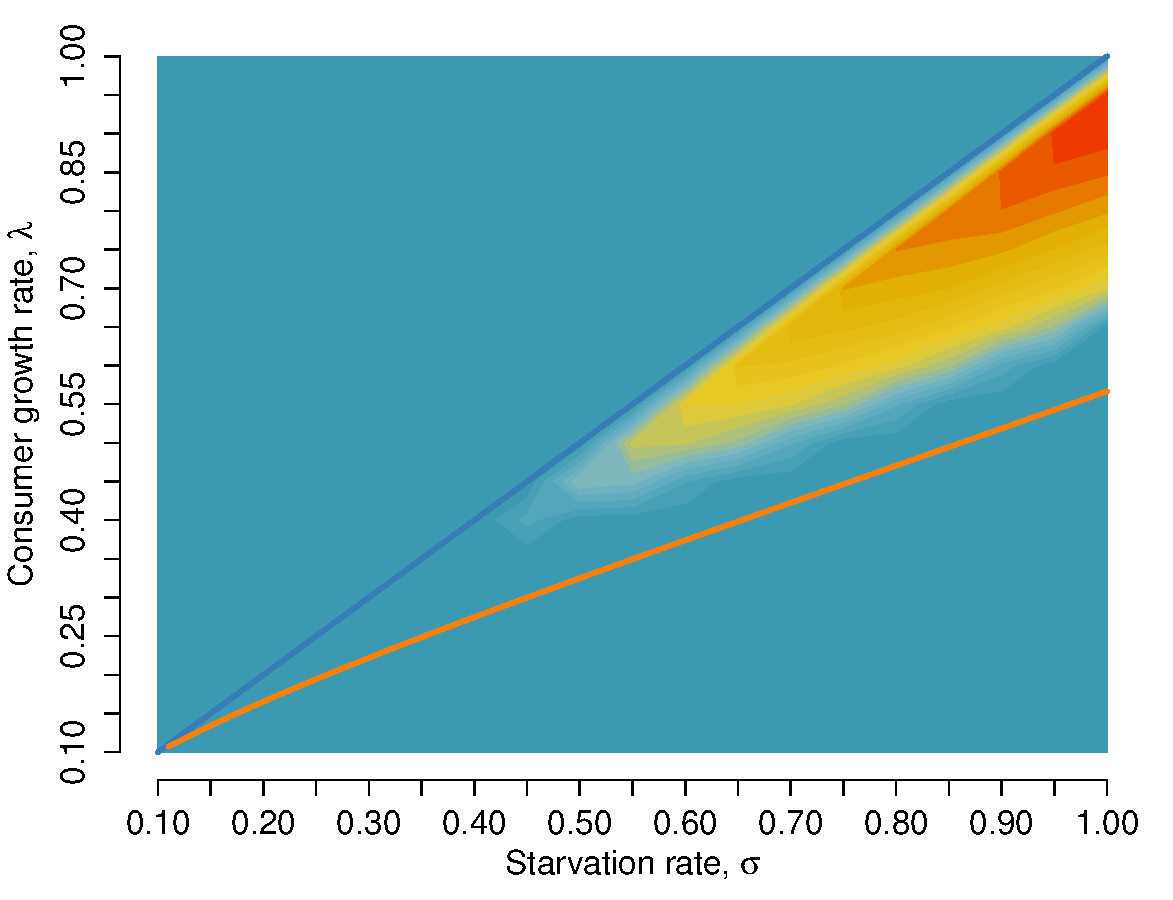
\includegraphics[width=0.5\textwidth]{fig_Hopf.pdf}
	\caption{
	Saddle Node bifurcation
	}
	\label{SN}
\end{figure}


\begin{figure}[h]
	\centering
	\includegraphics[width=0.5\textwidth]{fig_resvuln.pdf}
	\caption{
	Probability that the resource value is less than threshold = 0.05
	}
	\label{SN}
\end{figure}



\begin{figure}[h]
	\centering
	\includegraphics[width=0.5\textwidth]{fig_Competition.pdf}
	\caption{
	Hopf bifurcation
	}
	\label{SN}
\end{figure}






\end{document}
